%%%%%%%%%%%%%%%%%%%%%%%%%%%%%%%%%%%%%%%%%
% Beamer Presentation
% LaTeX Template
% Version 2.0 (March 8, 2022)
%
% This template originates from:
% https://www.LaTeXTemplates.com
%
% Author:
% Vel (vel@latextemplates.com)
%
% License:
% CC BY-NC-SA 4.0 (https://creativecommons.org/licenses/by-nc-sa/4.0/)
%
%%%%%%%%%%%%%%%%%%%%%%%%%%%%%%%%%%%%%%%%%

%----------------------------------------------------------------------------------------
%	PACKAGES AND OTHER DOCUMENT CONFIGURATIONS
%----------------------------------------------------------------------------------------

\documentclass[
	11pt, % Set the default font size, options include: 8pt, 9pt, 10pt, 11pt, 12pt, 14pt, 17pt, 20pt
	%t, % Uncomment to vertically align all slide content to the top of the slide, rather than the default centered
	%aspectratio=169, % Uncomment to set the aspect ratio to a 16:9 ratio which matches the aspect ratio of 1080p and 4K screens and projectors
]{beamer}

\graphicspath{{Images/}{./}} % Specifies where to look for included images (trailing slash required)

\usepackage{booktabs} % Allows the use of \toprule, \midrule and \bottomrule for better rules in tables
\usepackage{graphicx}
\usepackage{subcaption}
\newcommand\independent{\protect\mathpalette{\protect\independenT}{\perp}}
\def\independenT#1#2{\mathrel{\rlap{$#1#2$}\mkern2mu{#1#2}}}

%----------------------------------------------------------------------------------------
%	SELECT LAYOUT THEME
%----------------------------------------------------------------------------------------

% Beamer comes with a number of default layout themes which change the colors and layouts of slides. Below is a list of all themes available, uncomment each in turn to see what they look like.

%\usetheme{default}
%\usetheme{AnnArbor}
%\usetheme{Antibes}
%\usetheme{Bergen}
%\usetheme{Berkeley}
%\usetheme{Berlin}
%\usetheme{Boadilla}
%\usetheme{CambridgeUS}
%\usetheme{Copenhagen}
%\usetheme{Darmstadt}
%\usetheme{Dresden}
%\usetheme{Frankfurt}
%\usetheme{Goettingen}
\usetheme{Hannover}
%\usetheme{Ilmenau}
%\usetheme{JuanLesPins}
%\usetheme{Luebeck}
%\usetheme{Madrid}
%\usetheme{Malmoe}
%\usetheme{Marburg}
%\usetheme{Montpellier}
%\usetheme{PaloAlto}
%\usetheme{Pittsburgh}
%\usetheme{Rochester}
%\usetheme{Singapore}
%\usetheme{Szeged}
%\usetheme{Warsaw}

%----------------------------------------------------------------------------------------
%	SELECT COLOR THEME
%----------------------------------------------------------------------------------------

% Beamer comes with a number of color themes that can be applied to any layout theme to change its colors. Uncomment each of these in turn to see how they change the colors of your selected layout theme.

%\usecolortheme{albatross}
%\usecolortheme{beaver}
%\usecolortheme{beetle}
%\usecolortheme{crane}
%\usecolortheme{dolphin}
%\usecolortheme{dove}
%\usecolortheme{fly}
\usecolortheme{lily}
%\usecolortheme{monarca}
%\usecolortheme{seagull}
%\usecolortheme{seahorse}
%\usecolortheme{spruce}
%\usecolortheme{whale}
%\usecolortheme{wolverine}

%----------------------------------------------------------------------------------------
%	SELECT FONT THEME & FONTS
%----------------------------------------------------------------------------------------

% Beamer comes with several font themes to easily change the fonts used in various parts of the presentation. Review the comments beside each one to decide if you would like to use it. Note that additional options can be specified for several of these font themes, consult the beamer documentation for more information.

\usefonttheme{default} % Typeset using the default sans serif font
%\usefonttheme{serif} % Typeset using the default serif font (make sure a sans font isn't being set as the default font if you use this option!)
%\usefonttheme{structurebold} % Typeset important structure text (titles, headlines, footlines, sidebar, etc) in bold
%\usefonttheme{structureitalicserif} % Typeset important structure text (titles, headlines, footlines, sidebar, etc) in italic serif
%\usefonttheme{structuresmallcapsserif} % Typeset important structure text (titles, headlines, footlines, sidebar, etc) in small caps serif

%------------------------------------------------

%\usepackage{mathptmx} % Use the Times font for serif text
\usepackage{palatino} % Use the Palatino font for serif text

%\usepackage{helvet} % Use the Helvetica font for sans serif text
\usepackage[default]{opensans} % Use the Open Sans font for sans serif text
%\usepackage[default]{FiraSans} % Use the Fira Sans font for sans serif text
%\usepackage[default]{lato} % Use the Lato font for sans serif text

%----------------------------------------------------------------------------------------
%	SELECT INNER THEME
%----------------------------------------------------------------------------------------

% Inner themes change the styling of internal slide elements, for example: bullet points, blocks, bibliography entries, title pages, theorems, etc. Uncomment each theme in turn to see what changes it makes to your presentation.

%\useinnertheme{default}
\useinnertheme{circles}
%\useinnertheme{rectangles}
%\useinnertheme{rounded}
%\useinnertheme{inmargin}

%----------------------------------------------------------------------------------------
%	SELECT OUTER THEME
%----------------------------------------------------------------------------------------

% Outer themes change the overall layout of slides, such as: header and footer lines, sidebars and slide titles. Uncomment each theme in turn to see what changes it makes to your presentation.

%\useoutertheme{default}
%\useoutertheme{infolines}
%\useoutertheme{miniframes}
%\useoutertheme{smoothbars}
%\useoutertheme{sidebar}
%\useoutertheme{split}
%\useoutertheme{shadow}
%\useoutertheme{tree}
%\useoutertheme{smoothtree}

%\setbeamertemplate{footline} % Uncomment this line to remove the footer line in all slides
%\setbeamertemplate{footline}[page number] % Uncomment this line to replace the footer line in all slides with a simple slide count

%\setbeamertemplate{navigation symbols}{} % Uncomment this line to remove the navigation symbols from the bottom of all slides

%----------------------------------------------------------------------------------------
%	PRESENTATION INFORMATION
%----------------------------------------------------------------------------------------

\title[Model-X Knockoffs]{Model-X Knockoffs} % The short title in the optional parameter appears at the bottom of every slide, the full title in the main parameter is only on the title page

%\subtitle{Optional Subtitle} % Presentation subtitle, remove this command if a subtitle isn't required

\author[Chris Hemmens]{Christopher Hemmens} % Presenter name(s), the optional parameter can contain a shortened version to appear on the bottom of every slide, while the main parameter will appear on the title slide

\institute[]{\textit{chris@christopherhemmens.com}} % Your institution, the optional parameter can be used for the institution shorthand and will appear on the bottom of every slide after author names, while the required parameter is used on the title slide and can include your email address or additional information on separate lines

\date[12.12.2023]{PyData Lausanne Meetup - EPFL Innovation Park \\ 12th December 2023} % Presentation date or conference/meeting name, the optional parameter can contain a shortened version to appear on the bottom of every slide, while the required parameter value is output to the title slide

%----------------------------------------------------------------------------------------

\begin{document}

%----------------------------------------------------------------------------------------
%	TITLE SLIDE
%----------------------------------------------------------------------------------------

\begin{frame}
	\titlepage % Output the title slide, automatically created using the text entered in the PRESENTATION INFORMATION block above
\end{frame}

%----------------------------------------------------------------------------------------
%	TABLE OF CONTENTS SLIDE
%----------------------------------------------------------------------------------------

% The table of contents outputs the sections and subsections that appear in your presentation, specified with the standard \section and \subsection commands. You may either display all sections and subsections on one slide with \tableofcontents, or display each section at a time on subsequent slides with \tableofcontents[pausesections]. The latter is useful if you want to step through each section and mention what you will discuss.

\begin{frame}
	\frametitle{Presentation Overview} % Slide title, remove this command for no title
	
	\tableofcontents % Output the table of contents (all sections on one slide)
	%\tableofcontents[pausesections] % Output the table of contents (break sections up across separate slides)
\end{frame}

%----------------------------------------------------------------------------------------
%	PRESENTATION BODY SLIDES
%----------------------------------------------------------------------------------------

\section{About Me}

\begin{frame}
	\frametitle{About Me}
	
	\begin{itemize}
		\item Studied Mathematics with German at Imperial College, London.
		\item In 2017, completed a PhD in Finance at the University of Geneva as part of the Geneva Finance Research Institute where I specialised in statistical modelling, econometrics, behavioural economics, and asset pricing.
		\item Won the Swiss Finance Institute prize for Best Doctoral Paper in 2016.
	\end{itemize}
\end{frame}

\begin{frame}
	\frametitle{About Me}
	
	\begin{itemize}
		\item Became interested in data science and joined a tech startup in Geneva in 2018 where I learned to program in Python.
		\item Began freelancing as a data science consultant as part of the Toptal global platform in 2021 with whom I've worked on a range of data science and data engineering projects.
		\item For the last year, I've been doing research for HEIG-VD in Yverdon-les-Bains as part of a job placement scheme.
		\item Earned my Professional Data Engineer certification from Google Cloud in September 2023. 
	\end{itemize}
\end{frame}

\section{Model-X Knockoffs}

\begin{frame}
	\begin{itemize}
		\item Panning for Gold: Model-X Knockoffs for High-dimensional Controlled Variable Selection
		\begin{itemize}
			\item Cand\`{e}s, Fan, Janson, Lv
			\item Journal of the Royal Statistical Society Series B: Statistical Methodology 80, no. 3 (2018)
		\end{itemize}
		\bigskip
		\item Metropolized Knockoff Sampling
		\begin{itemize}
			\item Bates, Cand\`{e}s, Janson, Wang
			\item Journal of the American Statistical Association 116:535 (2021)
		\end{itemize}
		\bigskip
		\item New perspectives on knockoffs construction
		\begin{itemize}
			\item Berti, Dreassi, Leisen, Pratelli
			\item Journal of Statistical Planning and Inference 223 (2023)
		\end{itemize}
	\end{itemize}
\end{frame}

\subsection{Panning for Gold (2018)}

\begin{frame}
	\frametitle{Panning for Gold}
	
	\begin{center}
		\textbf{How can one control for the false discovery rate in high-dimensional non-linear models?}
		
		\bigskip
		
		What happens if you have more features than observations and yet you know that only a handful of them contain any explanatory power? For example, which genes affect a particular health outcome?
	\end{center}
\end{frame}

\begin{frame}
	\frametitle{Model-X Knockoffs}
	There are $n$ \textbf{independently and identically distributed} observations of $(X,Y)$ where
	
	$$X=(X_1,\dots,X_p)\in\mathbb{R}^p\text{ and }Y\in\mathbb{R}$$
	
	\bigskip
	
	A new family of random variables, $\tilde{X}=\left(\tilde{X}_1,\dots,\tilde{X}_p\right)$ is a knockoff of $X$ if
	
	\begin{enumerate}
		\item for any subset $S\subset\{1,\dots,p\}$, $$\left(X,\tilde{X}\right)_{\text{swap}(S)}\stackrel{d}{=}\left(X,\tilde{X}\right)$$
		\item $\tilde{X}\independent Y | X$ if there is a response $Y$.
	\end{enumerate}
\end{frame}

\begin{frame}
	\frametitle{Example}
	
	If $p=3$ and $S=\{2,3\}$, then
	
	$$\left(X_1,X_2,X_3,\tilde{X}_1,\tilde{X}_2,\tilde{X}_3\right)_{\text{swap}(\{2,3\})}\stackrel{d}{=}\left(X_1,\tilde{X}_2,\tilde{X}_3,\tilde{X}_1,X_2,X_3\right)$$
\end{frame}

\begin{frame}
	\frametitle{Normal $(0,\Sigma)$}
	Suppose 
	
	$$X\sim\mathcal{N}(0,\Sigma)$$
	\bigskip
	
	Then
	
	$$\left(X,\tilde{X}\right)\sim\mathcal{N}(0,\textbf{\textit{G}}),\text{  where  }\textbf{\textit{G}}=\left[\begin{array}{c c}
		\Sigma & \Sigma - D \\
		\Sigma - D & \Sigma
	\end{array}\right]$$
	
	\bigskip
	
	where $D$ is any diagonal matrix such that \textbf{\textit{G}} is positive semidefinite.
\end{frame}

\begin{frame}
	\frametitle{Sampling Knockoffs}
	
	It is now possible to sample the knockoffs, $\tilde{X}$, from the conditional distribution
	
	$$\tilde{X}|X\stackrel{d}{=}\mathcal{N}(\mu,\textbf{\textit{V}})$$
	
	\bigskip
	
	where
	
	$$\begin{array}{r c l}
		\mu & = & X-X\Sigma^{-1}D \\
		&& \\
		\textbf{\textit{V}} & = & 2D - D\Sigma^{-1}D
	\end{array}$$
\end{frame}

\begin{frame}
	\frametitle{What if Non-Gaussian?}
	
	\begin{tabular}{l}
		$j=1$ \textbf{while} $j\le p$ \textbf{do} \\
		 $|\text{     }$ Sample $\tilde{X}_j$ from $\mathcal{L}\left(X_j\left|X_{-j},\tilde{X}_{1:j-1}\right.\right)$ \\
		 $|\text{     }$ $j=j+1$ \\
		\textbf{end}
	\end{tabular}
	
	\bigskip
	
	For example, if $p=3$, sample $$\tilde{X}_1 \text{ from } \mathcal{L}(X_1|X_2,X_3)$$ then sample $$\tilde{X}_2 \text{ from } \mathcal{L}(X_2|X_1,X_3,\tilde{X}_1)$$ and so on and so forth.
\end{frame}

\begin{frame}
	\frametitle{Crohn's Disease}
	
	\textbf{Cand\`{e}s et al} use the \textbf{knockoff procedure} to identify \textbf{gene clusters} that predict \textbf{Crohn's Disease} and compare the results to the \textbf{WTCCC study} published in \textit{Nature} in 2007.
	
	\bigskip
	
	With $p=71,145$ and $n=14,708$, they're able to identify \textbf{18 gene clusters} that are predictive of Crohn's outcomes compared to \textbf{9 clusters} in the WTCCC paper.
	
\end{frame}

\subsection{Metropolized (2021)}

\begin{frame}
	\frametitle{Metropolis-Hastings}
	The Metropolis-Hastings algorithm (Metropolis et al 1953; Hastings 1970) provides a general \textbf{time-reversible Markov transition kernel} whose stationary distribution is an arbitrary density function $\pi$.
	
	\bigskip
	
	To construct a transition from $x$ to $y$, generate $x^*$ from a distribution $q(\cdot|x)$ and set
	
	$$y=\left\{\begin{array}{l c l}
		x^* && \text{with prob }\alpha \\
		x && \text{with prob }1-\alpha
	\end{array}\right.$$
	
	where
	
	$$\alpha=\min\left(1,\dfrac{\pi(x^*)q(x|x^*)}{\pi(x)q(x^*|x)}\right)$$
\end{frame}

\begin{frame}
	\frametitle{The Target Distribution}
	As in \textit{Panning for Gold}, the target distribution, i.e. $\pi$, is $$\mathcal{L}\left(X_j\left|X_{-j},\tilde{X}_{1:j-1}\right.\right).$$
	
	\bigskip
	
	However, the target density for this distribution cannot be evaluated because it depends on an integral over the proposal distribution, $x^*$. Hence, the target distribution, $\pi$, is set to be
	
	$$\mathcal{L}\left(X_j\left|X_{-j},\tilde{X}_{1:j-1},X^*_{1:j-1}\right.\right).$$
\end{frame}

\begin{frame}
	\frametitle{Metropolized Knockoff Sampling}
	
	\begin{tabular}{l}
		\textbf{for} $j=1$ \textbf{to} $p$ \textbf{do} \\
		$|\text{     }$ Sample $X^*_j=x^*_j$ from a faithful proposal distribution $q_j$. \\
		$|\text{     }$ Accept the proposal with probability \\
		$|\text{                         }$ ${\scriptstyle\min\left(1,\frac{q_j(x_j|x^*_j)\mathbb{P}\left(X_{-j}=x_{-j},X_j=x^*_j,\tilde{X}_{1:j-1}=\tilde{x}_{1:j-1},X^*_{1:j-1}=x^*_{1:j-1}\right)}{q_j(x^*_j|x_j)\mathbb{P}\left(X_{-j}=x_{-j},X_j=x_j,\tilde{X}_{1:j-1}=\tilde{x}_{1:j-1},X^*_{1:j-1}=x^*_{1:j-1}\right)}\right)}$ \\
		$|\text{     }$ Upon acceptance, set $\tilde{x}_j=x^*_j$; otherwise, set $\tilde{x}_j=x_j$. \\
		\textbf{end}
	\end{tabular}
\end{frame}

\begin{frame}
	\frametitle{Knockoff Quality}
	
	Using \textit{mean absolute correlation} as a measure of knockoff quality, where
	
	$$\text{MAC}\left(\mathcal{L}\left(X,\tilde{X}\right)\right):=\frac{1}{p}\sum_{j=1}^p \left|\text{corr}\left(X_j,\tilde{X}_j\right)\right|$$
	
	\bigskip
	
	the Metropolized Knockoff Sampling algorithm takes \textbf{significantly longer to run} but results in knockoffs of \textbf{higher quality}.
\end{frame}

\subsection{New perspectives (2023)}

\begin{frame}
	\frametitle{Knockoffs from Copulas}
	
	Suppose $F$ and $F_i$ are the distribution functions of $X$ and $X_i$ respectively.
	
	\bigskip
	
	By \textit{Sklar's Theorem}, there is a $p$-copula $C$ such that, $\forall x\in\mathbb{R}^p$,
	
	$$F(x) = C\left[F_1(x_1),\dots,F_p(x_p)\right]$$
	
	\bigskip
	
	Then, for any symmetric 2-copulas $D_1,\dots,D_p$, $\forall x\in\mathbb{R}^{2p}$,
	
	$$H(x)=C\left[D_1\left(F_1(x_1),F_1(x_{p+1})\right),\dots,D_p\left(F_p(x_p),F_p(x_{2p})\right)\right]$$
	
	is a candidate for the distribution function of $(X,\tilde{X})$.
\end{frame}

\begin{frame}
	\frametitle{Is H a distribution function?}
	
	$H$ is a distribution function on $\mathbb{R}^{2p}$ whenever
	
	\begin{enumerate}
		\item $D_i$ is of class $C^2$ for each $i\in I$;
		\item $C$ has a density $\varphi$ with respect to $m_p$, the Lebesgue measure on the Borel $\sigma$-field on $\mathbb{R}^p$;
		\item $\varphi$ is of class $C^p$ and, at each point $u\in[0,1]^{2p}$, one obtains
	\end{enumerate}
	$${\scriptstyle \frac{\partial^p}{\partial u_{2p}\dots\partial u_{p+1}}\varphi\left[D_1(u_1,u_{p+1}),\dots,D_p(u_p,u_{2p})\right]\prod_{i=1}^{p}\frac{\partial}{\partial u_i}D_i(u_i,u_{p+i})\ge 0}$$
\end{frame}

\begin{frame}
	\frametitle{Copula Knockoffs General Algorithm}
	1. Choose $F_1,\dots,F_p$ on $\mathbb{R}$, a $p$-copula $C$ and a family of 2-copulas $D_1,\dots,D_p$ in such a way that
	
	$$H(x,\tilde{x})=C\left[D_1\left(F_1(x_1),F_1(\tilde{x}_1)\right),\dots,D_p\left(F_p(x_p),F_p(\tilde{x}_p)\right)\right]$$
	
	is a distribution function on $\mathbb{R}^{2p}$.
	
	2. Sample $\tilde{x}$ from the conditional density
	
	$$p(\tilde{x}|x)=\frac{1}{\varphi[F_1(x_1),\dots,F_p(x_p)]\prod_{i=1}^p f_i(x_i)}$$ $$\times\frac{\partial^{2p}H}{\partial x_p\dots\partial x_1\partial\tilde{x}_p\dots\partial\tilde{x}_1}(x,\tilde{x})$$
	
	where $\varphi$ and $f_i$ are the densities of $C$ and $F_i$ respectively.
\end{frame}

\begin{frame}
\frametitle{Copula Metropolis-Hastings Sampler}
1. Choose the initial value $\tilde{x}^{(0)}$

2. Choose the proposal distribution $K(\cdot|x)$

	\textbf{for} $j=1$ \textbf{to} $M$ \textbf{do}
	
	3. Sample $y$ from the proposal $K(\cdot|\tilde{x}^{(j-1)})$
	
	4. Compute acceptance probability 
	
	$$\alpha(\tilde{x}^{(j-1)},y)=\min\left\{\dfrac{\frac{\partial^{2p}H}{\partial x_p\dots\partial x_1\partial\tilde{x}_p\dots\partial\tilde{x}_1}(x,y)}{\frac{\partial^{2p}H}{\partial x_p\dots\partial x_1\partial\tilde{x}_p\dots\partial\tilde{x}_1}(x,\tilde{x}^{(j-1)})}\dfrac{K(\tilde{x}^{(j-1)}|y)}{K(y|\tilde{x}^{(j-1)})}\right\}$$
	
	5. Set $\tilde{x}^{(j)}=y$ with probability $\alpha(\tilde{x}^{(j-1)},y)$ and $\tilde{x}^{(j)}=\tilde{x}^{(j-1)}$ with probability $1-\alpha(\tilde{x}^{(j-1)},y)$.
	
	\textbf{end}

6. Return the sample $\tilde{x}^{(j)}$, $j=1,\dots,M$
\end{frame}

\section{Linear Algebra}

\subsection{Methodology}

\begin{frame}
	\frametitle{The Challenge}
	
	We observe
	
	$$\mathcal{X}\equiv(X_1,\dots,X_p)\in\mathbb{R}^{p\times n}$$
	
	where 
	
	$p$ is the number of features and
	
	$n$ is the number of observations.
	
	\bigskip
	
	We want to create
	
	$$\tilde{\mathcal{X}}\equiv(\tilde{X}_1,\dots,\tilde{X}_p)\in\mathbb{R}^{p\times n}$$
	
	such that $\tilde{\mathcal{X}}$ is a set of valid knockoffs for $\mathcal{X}$.
\end{frame}

\begin{frame}
	\frametitle{The Constraints}
	If $$\mu_{m,k}(X_i,X_j)$$ is the $m$th co-moment between features $i$ and $j$ with balance parameter $k<m$, then for $$2\le m\le 4\text{ and }1 \le k\le (m-1)$$ our constraints are

	\begin{itemize}
		\item $\tilde{X}_i \stackrel{d}{=} X_i, \,\, \forall i$
		\item $\mu_{m,k}(\tilde{X}_i,X_j)=\mu_{m,k}(X_i,X_j),\,\, \forall i\ne j$
		\item $\mu_{m,k}(\tilde{X}_i,\tilde{X}_j)=\mu_{m,k}(X_i,X_j),\,\, \forall i\ne j$
	\end{itemize}
\end{frame}

\begin{frame}
	\frametitle{The Optimisation}
	
	I tell the program to minimise the \textbf{summed squared correlation} between each feature and its knockoff:
	
	$$\sum_{i=1}^p \left(\mu_{2,1}(\tilde{X}_i,X_i)\right)^2$$
	
	subject to the constraints given.
	
	\bigskip
	
	To reduce the computation time as much as possible, I estimate the multivariate distribution using a Gaussian copula:
	
	$$\Phi\left(\Phi^{-1}\left(F_1(X_1),\dots,F_p(X_p)\right)\right)$$
	
	and use the methodology set out in Cand\`{e}s et al (2018) to generate an initial guess. 
\end{frame}

\subsection{Model Tests}

\begin{frame}
	\frametitle{Artificial Features}
	To test the algorithm, I sample \textbf{four Normal(0,1)} random variables with \textbf{100 observations} each. I then shuffle them to artificially generate non-zero correlation, coskewness, and cokurtosis as follows
	
	\begin{itemize}
		\item Feature 1 has \textbf{smaller} observations shuffled towards the end of the sample,
		\item Feature 2 has \textbf{larger} observations shuffled towards the end of the sample,
		\item Feature 3 has observations \textbf{close to the mean} shuffled towards the end of the sample,
		\item Feature 4 is left \textbf{unshuffled}.
	\end{itemize}
	
	I run the algorithm for up to \textbf{20 iterations}.
	
\end{frame}

\begin{frame}
	\frametitle{Model Performance}
\begin{figure}
	\centering
	\begin{subfigure}{0.3\textwidth}
		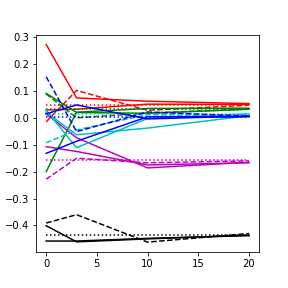
\includegraphics[width=\textwidth]{Graph03_2_2_1}
		\caption{Correlation}
	\end{subfigure}
	\hfill
	\begin{subfigure}{0.6\textwidth}
		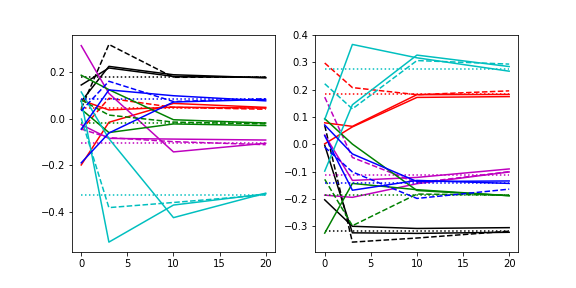
\includegraphics[width=\textwidth]{Graph03_2_2_2}
		\caption{Coskewness}
	\end{subfigure}
	\hfill
	\begin{subfigure}{\textwidth}
		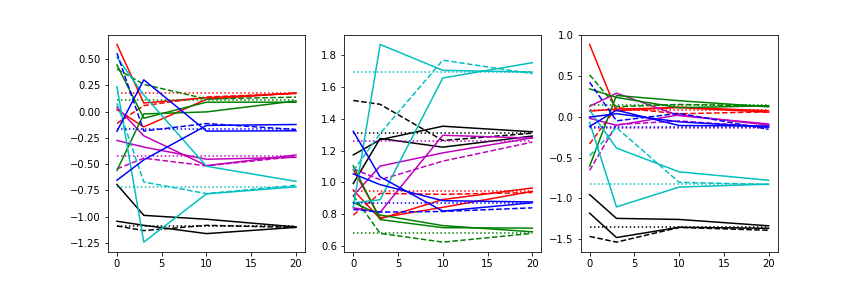
\includegraphics[width=\textwidth]{Graph03_2_2_3}
		\caption{Cokurtosis}
	\end{subfigure}
\end{figure}
\end{frame}

\begin{frame}
\frametitle{More Parameters}
\begin{figure}
	\centering
	\begin{subfigure}{0.45\textwidth}
		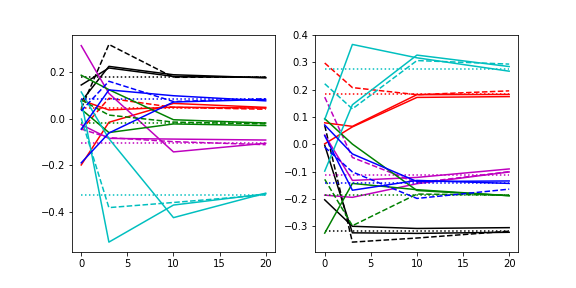
\includegraphics[width=\textwidth]{Graph03_2_2_2}
		\caption{$p=4$, $n=100$; -:--:26}
	\end{subfigure}
	\begin{subfigure}{0.45\textwidth}
		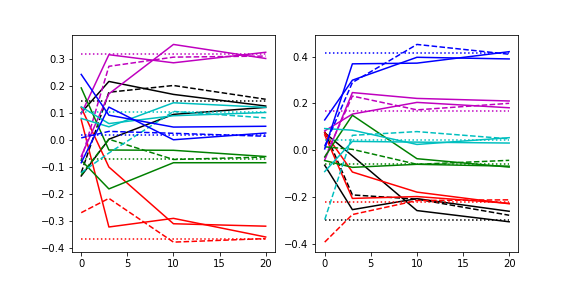
\includegraphics[width=\textwidth]{Graph03_3_2_2}
		\caption{$p=8$, $n=100$; -:01:27}
	\end{subfigure}
	\begin{subfigure}{0.45\textwidth}
		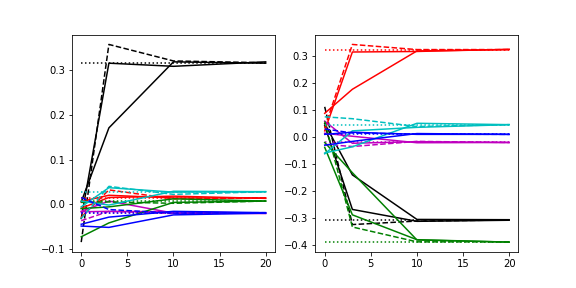
\includegraphics[width=\textwidth]{Graph03_2_3_2}
		\caption{$p=4$, $n=1000$; -:12:40}
	\end{subfigure}
	\begin{subfigure}{0.45\textwidth}
		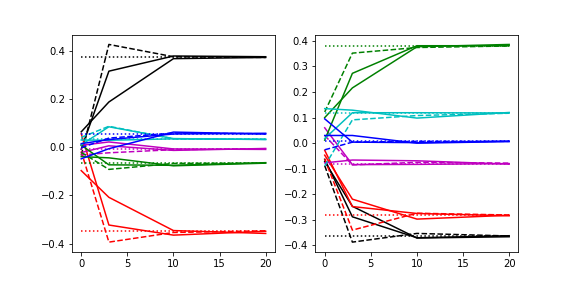
\includegraphics[width=\textwidth]{Graph03_3_3_2}
		\caption{$p=8$, $n=1000$; 1:26:15}
	\end{subfigure}
\end{figure}
\end{frame}

\begin{frame}
	\frametitle{Distributions and Correlations}
	
	\begin{tabular}{c | c c}
		Worst outcome & Dist. p-value & Corr. with Feature \\
		\hline
		&&\\
		$p=4$, $n=100$ & 35.8\% & 0.185 \\
		$p=4$, $n=1000$ & 12.9\% & 0.080 \\
		$p=8$, $n=100$ & 36.9\% & 0.298 \\
		$p=8$, $n=1000$ & 6.4\% & 0.099 \\
	\end{tabular}
\end{frame}

\subsection{Real Data}

\begin{frame}
	\frametitle{Stock Data}
	I take daily returns data from the Swiss Market Index for the \textbf{20 constituents} for the period 26th May 2017 to the 8th April 2019. This sample contains \textbf{481 observations}.
	
	\bigskip
	
	I \textbf{scale} the returns so that they all have \textbf{mean 0} and \textbf{variance 1} and then estimate the joint distribution using a Gaussian copula.
	
	\bigskip
	
	This process identifies that the univariate distributions of all the stocks are \textbf{student-t} with degrees of freedom ranging from 3.08 to 5.81.
\end{frame}

\begin{frame}
	\frametitle{Results}
	I run the algorithm for \textbf{100 iterations} for a total time of \textbf{13:37:27}.
	
	\bigskip
	
	Quartiles of the \textbf{20} target variables:
	
	\bigskip
	
	\begin{center}
		\begin{tabular}{r | c c c c c}
			Quartile & Min & 0.25 & 0.50 & 0.75 & Max \\
			& Lonza &&&& UBS \\
			\hline
			Corr. & 0.36 & 0.51 & 0.60 & 0.71 & 0.92
		\end{tabular}
	\end{center}
\end{frame}

\begin{frame}
	\frametitle{Contrainst Adherence}
	\begin{table}
		\centering
		\tiny
		\begin{tabular}{r r | c | c c || c | c c}
			& & \multicolumn{3}{c}{Nestl\'{e}} & \multicolumn{3}{c}{UBS} \\
			& & Real & Feature & Knockoff & Real & Feature & Knockoff \\
			\hline
			&&&&&&& \\
			Lonza & Correlation & 0.364 & 0.366 & 0.365 & 0.424 & 0.424 & 0.424 \\
			\hline
			&&&&&&& \\
			& Left Coskewness & -0.030 & -0.026 & -0.030 & -0.122 & -0.122 & -0.120 \\
			& Right Coskewness & -0.155 & -0.157 & -0.157 & -0.273 & -0.274 & -0.275 \\
			\hline
			&&&&&&& \\
			& Left Cokurtosis & 1.181 & 1.178 & 1.179 & 1.642 & 1.643 & 1.643 \\
			& Central Cokurtosis & 1.579 & 1.577 & 1.574 & 1.871 & 1.872 & 1.875 \\
			& Right Cokurtosis & 1.417 & 1.432 & 1.420 & 1.811 & 1.805 & 1.807 \\
			\hline
			\hline
			&&&&&&& \\
			Nestl\'{e} & Correlation & & & & 0.337 & 0.336 & 0.336 \\
			\hline
			&&&&&&& \\
			& Left Coskewness & & & & -0.136 & -0.134 & -0.136 \\
			& Right Coskewness & & & & -0.233 & -0.237 & -0.236 \\
			\hline
			&&&&&&& \\
			& Left Cokurtosis & & & & 1.599 & 1.596 & 1.605 \\
			& Central Cokurtosis & & & & 1.793 & 1.796 & 1.786 \\
			& Right Cokurtosis & & & & 1.437 & 1.434 & 1.444 \\
		\end{tabular}
	\end{table}
\end{frame}

%\section{Text Examples} % Sections are added in order to organize your presentation into discrete blocks, all sections and subsections are automatically output to the table of contents as an overview of the talk but NOT output in the presentation as separate slides
%
%%------------------------------------------------
%
%\subsection{Paragraphs and Lists}
%
%\begin{frame}
%	\frametitle{Paragraphs of Text}
%	
%	Sed iaculis \alert{dapibus gravida}. Morbi sed tortor erat, nec interdum arcu. Sed id lorem lectus. Quisque viverra augue id sem ornare non aliquam nibh tristique. Aenean in ligula nisl. Nulla sed tellus ipsum. Donec vestibulum ligula non lorem vulputate fermentum accumsan neque mollis.
%	
%	\bigskip % Vertical whitespace
%	
%	% Quote example
%	\begin{quote}
%		Sed diam enim, sagittis nec condimentum sit amet, ullamcorper sit amet libero. Aliquam vel dui orci, a porta odio.\\
%		--- Someone, somewhere\ldots
%	\end{quote}
%	
%	\bigskip % Vertical whitespace
%	
%	Nullam id suscipit ipsum. Aenean lobortis commodo sem, ut commodo leo gravida vitae. Pellentesque vehicula ante iaculis arcu pretium rutrum eget sit amet purus. Integer ornare nulla quis neque ultrices lobortis.
%\end{frame}
%
%%------------------------------------------------
%
%\begin{frame}
%	\frametitle{Lists}
%	\framesubtitle{Bullet Points and Numbered Lists} % Optional subtitle
%	
%	\begin{itemize}
%		\item Lorem ipsum dolor sit amet, consectetur adipiscing elit
%		\item Aliquam blandit faucibus nisi, sit amet dapibus enim tempus
%		\begin{itemize}
%			\item Lorem ipsum dolor sit amet, consectetur adipiscing elit
%			\item Nam cursus est eget velit posuere pellentesque
%		\end{itemize}
%		\item Nulla commodo, erat quis gravida posuere, elit lacus lobortis est, quis porttitor odio mauris at libero
%	\end{itemize}
%	
%	\bigskip % Vertical whitespace
%	
%	\begin{enumerate}
%		\item Nam cursus est eget velit posuere pellentesque
%		\item Vestibulum faucibus velit a augue condimentum quis convallis nulla gravida 
%	\end{enumerate}
%\end{frame}
%
%%------------------------------------------------
%
%\subsection{Blocks}
%
%\begin{frame}
%	\frametitle{Blocks of Highlighted Text}
%	
%	\begin{block}{Block Title}
%		Lorem ipsum dolor sit amet, consectetur adipiscing elit. Integer lectus nisl, ultricies in feugiat rutrum, porttitor sit amet augue.
%	\end{block}
%	
%	\begin{exampleblock}{Example Block Title}
%		Aliquam ut tortor mauris. Sed volutpat ante purus, quis accumsan.
%	\end{exampleblock}
%	
%	\begin{alertblock}{Alert Block Title}
%		Pellentesque sed tellus purus. Class aptent taciti sociosqu ad litora torquent per conubia nostra, per inceptos himenaeos.
%	\end{alertblock}
%	
%	\begin{block}{} % Block without title
%		Suspendisse tincidunt sagittis gravida. Curabitur condimentum, enim sed venenatis rutrum, ipsum neque consectetur orci.
%	\end{block}
%\end{frame}
%
%%------------------------------------------------
%
%\subsection{Columns}
%
%\begin{frame}
%	\frametitle{Multiple Columns}
%	\framesubtitle{Subtitle} % Optional subtitle
%	
%	\begin{columns}[c] % The "c" option specifies centered vertical alignment while the "t" option is used for top vertical alignment
%		\begin{column}{0.45\textwidth} % Left column width
%			\textbf{Heading}
%			\begin{enumerate}
%				\item Statement
%				\item Explanation
%				\item Example
%			\end{enumerate}
%		\end{column}
%		\begin{column}{0.5\textwidth} % Right column width
%			Lorem ipsum dolor sit amet, consectetur adipiscing elit. Integer lectus nisl, ultricies in feugiat rutrum, porttitor sit amet augue. Aliquam ut tortor mauris. Sed volutpat ante purus, quis accumsan dolor.
%		\end{column}
%	\end{columns}
%\end{frame}
%
%%------------------------------------------------
%
%\section{Table and Figure Examples}
%
%\subsection{Table}
%
%\begin{frame}
%	\frametitle{Table}
%	\framesubtitle{Subtitle} % Optional subtitle
%	
%	\begin{table}
%		\begin{tabular}{l l l}
%			\toprule
%			\textbf{Treatments} & \textbf{Response 1} & \textbf{Response 2}\\
%			\midrule
%			Treatment 1 & 0.0003262 & 0.562 \\
%			Treatment 2 & 0.0015681 & 0.910 \\
%			Treatment 3 & 0.0009271 & 0.296 \\
%			\bottomrule
%		\end{tabular}
%		\caption{Table caption}
%	\end{table}
%\end{frame}
%
%%------------------------------------------------
%
%%\subsection{Figure}
%%
%%\begin{frame}
%%	\frametitle{Figure}
%%	
%%	\begin{figure}
%%		\includegraphics[width=0.8\linewidth]{creodocs_logo.pdf}
%%		\caption{Creodocs logo.}
%%	\end{figure}
%%\end{frame}
%
%%------------------------------------------------
%
%\section{Mathematics}
%
%\begin{frame}
%	\frametitle{Definitions \& Examples}
%	
%	\begin{definition}
%		A \alert{prime number} is a number that has exactly two divisors.
%	\end{definition}
%	
%	\smallskip % Vertical whitespace
%	
%	\begin{example}
%		\begin{itemize}
%			\item 2 is prime (two divisors: 1 and 2).
%			\item 3 is prime (two divisors: 1 and 3).
%			\item 4 is not prime (\alert{three} divisors: 1, 2, and 4).
%		\end{itemize}
%	\end{example}
%	
%	\smallskip % Vertical whitespace
%	
%	You can also use the \texttt{theorem}, \texttt{lemma}, \texttt{proof} and \texttt{corollary} environments.
%\end{frame}
%
%%------------------------------------------------
%
%\begin{frame}
%	\frametitle{Theorem, Corollary \& Proof}
%	
%	\begin{theorem}[Mass--energy equivalence]
%		$E = mc^2$
%	\end{theorem}
%	
%	\begin{corollary}
%		$x + y = y + x$
%	\end{corollary}
%	
%	\begin{proof}
%		$\omega + \phi = \epsilon$
%	\end{proof}
%\end{frame}
%
%%------------------------------------------------
%
%\begin{frame}
%	\frametitle{Equation}
%
%	\begin{equation}
%		\cos^3 \theta =\frac{1}{4}\cos\theta+\frac{3}{4}\cos 3\theta
%	\end{equation}
%\end{frame}
%
%%------------------------------------------------
%
%\begin{frame}[fragile] % Need to use the fragile option when verbatim is used in the slide
%	\frametitle{Verbatim}
%	
%	\begin{example}[Theorem Slide Code]
%		\begin{verbatim}
%			\begin{frame}
%				\frametitle{Theorem}
%				\begin{theorem}[Mass--energy equivalence]
%					$E = mc^2$
%				\end{theorem}
%		\end{frame}\end{verbatim} % Must be on the same line
%	\end{example}
%\end{frame}
%
%%------------------------------------------------
%
%\begin{frame}
%	Slide without title.
%\end{frame}
%
%%------------------------------------------------
%
%\section{Referencing}
%
%\begin{frame}
%	\frametitle{Citing References}
%	
%	An example of the \texttt{\textbackslash cite} command to cite within the presentation:
%	
%	\bigskip % Vertical whitespace
%	
%	This statement requires citation \cite{p1,p2}.
%\end{frame}
%
%%------------------------------------------------
%
%\begin{frame} % Use [allowframebreaks] to allow automatic splitting across slides if the content is too long
%	\frametitle{References}
%	
%	\begin{thebibliography}{99} % Beamer does not support BibTeX so references must be inserted manually as below, you may need to use multiple columns and/or reduce the font size further if you have many references
%		\footnotesize % Reduce the font size in the bibliography
%		
%		\bibitem[Smith, 2022]{p1}
%			John Smith (2022)
%			\newblock Publication title
%			\newblock \emph{Journal Name} 12(3), 45 -- 678.
%			
%		\bibitem[Kennedy, 2023]{p2}
%			Annabelle Kennedy (2023)
%			\newblock Publication title
%			\newblock \emph{Journal Name} 12(3), 45 -- 678.
%	\end{thebibliography}
%\end{frame}

%----------------------------------------------------------------------------------------
%	ACKNOWLEDGMENTS SLIDE
%----------------------------------------------------------------------------------------

\begin{frame}
	\frametitle{Acknowledgements}
	
\begin{center}
	Thank you to
	
	\textbf{Prof. Stephan Robert}
	
	of the 
	
	\textbf{Statistical Learning Research Group}
	
	based at
	
	\textbf{HEIG-VD, Yverdon-les-Bains}
\end{center}
\end{frame}

%----------------------------------------------------------------------------------------
%	CLOSING SLIDE
%----------------------------------------------------------------------------------------

\begin{frame}[plain] % The optional argument 'plain' hides the headline and footline
	\begin{center}
		{\Huge The End}
		
		\bigskip\bigskip % Vertical whitespace
		
		{\LARGE Questions? Comments?}
	\end{center}
\end{frame}

%----------------------------------------------------------------------------------------

\end{document} 